\chapter{Pointers}

As you know, pointers are one of the main features of the C programming languages, and ultimately one that makes it such a popular language for low-level programming, since pointers allow us to access specific memory regions directly. They are, however, also one of the most common sources of bugs and errors in C programs, and can easily lead to the failure of a complete system. 

Therefore, ACSL has some special constructs we can use for expressing specifications that include pointers. 

Let's have a look at a simple example again. Assume we want to write a function \textbf{swap}, which takes two pointers to integer variables as input and swaps the values that are saved at these locations:

\ceditor{swap.c}{code/pointers/swap_simple.c}

So let's think for a moment what kind of contract we need for such a function. We already know from the last chapter that we need to specify at least a postcondition we want to prove. In case of the \textbf{swap} function that might look something like this:

\ceditor{swap.c}{code/pointers/swap_post.c}

This introduces a new ACSL keyword that is very important. We can use \textbf{\textbackslash old} in a postcondition to refer to the value of a variable at the beginning of the function. That is an important concept, since the value of a variable (especially when dealing with pointers) might change during the execution of the function we are trying to specify. 

We can also see in this example, that we can combine multiple postconditions by using \mintinline{c}{&&} (similarly you can use \mintinline{c}{||} if you need it). Instead of using a logical AND, we could have also just written two separate ensures clauses. Both of them would work. 

If we try to use Frama-C on our contract, it actually looks a bit dire:

\begin{center}
    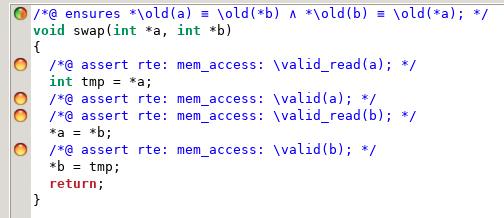
\includegraphics[width=0.6\textwidth]{images/frama_c_swap_post.png}
\end{center}

The guards that the RTE plugin inserted give us a hint as to why Frama-C could not prove our contract. We never said anything about the pointers \mintinline{c}{*a} and \mintinline{c}{*b}. What would happen if we did something like \mintinline{c}{swap(NULL, NULL)}?

So in order for Frama-C to know that we are not calling \textbf{swap} with any invalid pointer, we need to have a precondition:

\ceditor{swap.c}{code/pointers/swap_pre.c}

The ACSL keyword \textbf{\textbackslash valid} allows us to specify a guarantee that the provided pointer is valid. There is also a \textbf{\textbackslash valid\textunderscore read} which specifies that we can read from the given pointer, but we cannot write to it. That might be interesting for example when you want to read out certain configuration registers that are actually hardwired or can only be set during the boot up process. 

So with our \textbf{\textbackslash valid} precondition in place, we can finally prove the correctness of \textbf{swap}:

\begin{center}
    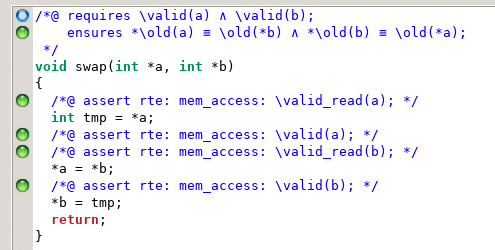
\includegraphics[width=0.5\textwidth]{images/frama_c_swap_pre.png}
\end{center}

But is this specification actually complete? If we would try a similar main function as we did in the previous chapter, we would see that Frama-C cannot prove that our \textbf{swap} function does not alter any global memory besides the two provided pointers. We again have to specify concretely, which locations our function can alter with the ACSL assigns statement:

\ceditor{swap.c}{code/pointers/swap.c}

As we will see later, the \textbf{\textbackslash valid} and \textbf{\textbackslash valid\textunderscore read} functions provided by ACSL are not only important when dealing with simple pointers. We will encounter them again when we talk about proving code that deals with arrays, since an array can also be seen as a collection of pointers to its elements. 

\section{Exercises}

\subsection{Max-pointer function}

Suppose we want to implement a function \textbf{max\textunderscore ptr} which takes two pointers to integer values as arguments and puts the bigger value at the first location and the smaller one at the second: 

\ceditor{max\textunderscore ptr.c}{exercises/pointers/max_ptr.c}

Write the required contract so that Frama-C can prove all assertions in the main function! 

\subsection{Decrementing integer by another integer}

Have a look at the following implementation of a decrement function:

\ceditor{decr\textunderscore by.c}{exercises/pointers/decr_by.c}

We provide two pointers to integers as input and the function \textbf{decr\textunderscore by} shall subtract the value the second pointer points to from the first one. Try writing a contract for this function. You will realize, that Frama-C actually fails to prove your postconditions. This is due to the possibility of aliasing. Two pointers can actually point to the same memory location. But what would happen if we did something like \mintinline{c}{int a = 5; decr_by(&a, &a)}? We have to tell Frama-C in a precondition that the two pointers are actually different, which we can do like this: \mintinline{c}{requires \separated (x, y);}. Try proving your function contract again, now it should be able to prove it correct. 

\subsection{Adding of pointed values}

In this exercise we want to create a function that takes two integer pointers as input and returns the sum of the values they point to:

\ceditor{add\textunderscore ptr.c}{exercises/pointers/add_ptr.c}

Implement the function \textbf{add\textunderscore ptr} and write the required pre- and postconditions to prove the assertion in the main function and the automatically generated run-time exceptions within \textbf{add\textunderscore ptr}! Do we need to use \textbf{\textbackslash separated} here? 
